\documentclass{article}
\usepackage{amsmath}
\usepackage{ctex}
\usepackage{graphicx}
\usepackage[utf8]{inputenc}
\usepackage{geometry}
\usepackage{pdfpages}
\usepackage{hyperref}
\hypersetup{hypertex=true,
            colorlinks=true,
            linkcolor=blue,
            anchorcolor=blue,
            citecolor=blue}
%以下是为了展示python代码引入的包
\usepackage{listings}
\usepackage{color}
\usepackage{float} %指定图片位置
\usepackage{subfigure}%并排子图 共享标题 有子标题
\usepackage{caption}
\usepackage{amssymb}
\usepackage{booktabs}
\usepackage{array}
\usepackage{makecell,rotating,multirow,diagbox}
\definecolor{dkgreen}{rgb}{0,0.6,0}
\definecolor{gray}{rgb}{0.5,0.5,0.5}
\definecolor{mauve}{rgb}{0.58,0,0.82}

\lstset{frame=tb,
  language=Python,
  aboveskip=3mm,
  belowskip=3mm,
  showstringspaces=false,
  columns=flexible,
  basicstyle={\small\ttfamily},
  numbers=none,
  numberstyle=\tiny\color{gray},
  keywordstyle=\color{blue},
  commentstyle=\color{dkgreen},
  stringstyle=\color{mauve},
  breaklines=true,
  breakatwhitespace=true,
  tabsize=3
}
%以上是为了展示python代码引入的包

\geometry{a4paper,scale=0.79}
\date{}
\title{神经网络模型报告文档4.10}
\author{许敬然}
\begin{document}
\maketitle

\section*{网络基本情况说明}

网络模型的目的是替代传统优化手段,更快速地完成参数反演。在已知血药浓度的时间离散点时,利用该模型可以快速得到一个机器学习意义上最可能与之相对应的三个参数(DSC<角质层中的有效扩散系数>、PFO<毛囊的渗透系数>、u1<由脱屑而向皮肤表面转移的速度>)。
从接收输入到输出结果,网络模型的工作时间大概为$\alpha \alpha \alpha \alpha \mbox{待填补}\alpha \alpha \alpha \alpha $。

网络的输入是形状为N*68的二维数组,其中“N”代表输入数据的条目数,“68”代表68个时间采样点。输入数据代表的是抽血采样得到的血药浓度。
网络的输出是形状为N*3的二维数组,其中“N”代表输出数据的条目数,“3”代表3个反演参数。
网络的架构是由全连接层和LayerNormalization层构成的共30层的残差网络。

在网络训练中,数据集的标签(label)是经过各种方式在参数空间的合理范围内取得的三参数组,数据集的特征(feature)是将标签中的三参数代入至BPTK模型计算得到的血药浓度曲线在68个时间点的取样。
(取样规则:从0.5时至20时结束,每0.5小时取一次样;从20.5时至74.5时结束,每2小时取一次样。总共得到68个时间取样点。)
损失函数设置为标签三参数和模型输出的三参数的MSE。

\section*{评价指标说明}

为了能更好地评价输出结果的拟合程度,除了损失函数外,还使用了能度量“原始标签参数代入至BPTK模型计算得到的血药浓度曲线”和“模型输出参数代入至BPTK模型计算得到的血药浓度曲线”之间差异的评价指标
(简称两个曲线分别为原始曲线与模型曲线)。
\subsection*{1.标签参数与网络输出参数的MSE}
简称为\textbf{loss}。该指标沿用了模型训练中的损失函数,即单组标签三参数和单组模型输出三参数的MSE(若有多组,取平均)。
\subsection*{2.标签参数与网络输出参数的相对误差数组的平均}
简称为\textbf{标签MRE}。该指标是一个含有三个元素的一维数组,是标签参数逐元素与网络输出参数计算相对误差的结果(若有多组,取平均)。
\subsection*{3.原始曲线与模型曲线之间的绝对误差的平均值}
简称为\textbf{MAE}。单组的原始曲线与模型曲线本质上是两个含有15000个元素的一维数组(共15000个时间戳),该指标即为两个数组之间绝对误差的平均(若有多组,取平均)。
\subsection*{4.原始曲线与模型曲线之间的相对误差的平均值}
简称为\textbf{MRE}。类似上一条,该指标即为两个数组之间相对误差的平均值(若有多组,取平均)。但该指标不稳定,在其他指标描述的效果很好的情况下,该指标可能会很高。
如图\ref{fig1},从可视化角度看,两条曲线是极为接近的,但是MRE却有49.775\%。原因可能是在计算相对误差时,分母的数值十分小,导致了相对误差指标描述能力的失真,尤其是在曲线的末端,血药浓度接近于0,失真效应就更强了。
\begin{figure}[H]
    \centering
    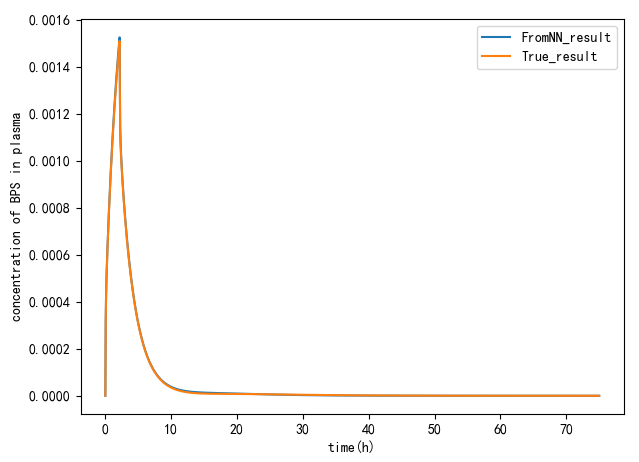
\includegraphics[scale=0.4]{p1-1.png}
    \caption{某组数据集外的三参数生成的原始曲线与模型曲线}
    \label{fig1}
\end{figure}
\subsection*{5.决定系数$R^2$}
简称为\textbf{$R^2$}。该指标原用于评价线性回归模型的拟合程度,但用于非线性的拟合模型时也可提供一个拟合程度的大致度量。
$R^2\in(0,1]$,越接近1说明拟合程度越好(若有多组,取平均)。
它的公式是$ R^2 = 1 - \frac{\text{ESS}}{\text{TSS}} = \frac{\text{RSS}}{\text{TSS}}$,其中$\text{ESS} = \sum_{i=1}^{n} (y_i - \hat{y}_i)^2$、 
$ \text{RSS} = \sum_{i=1}^{n} (\hat{y}_i - \bar{y})^2 $。
\subsection*{6.原始曲线与模型曲线之间修正后的绝对误差的平均值}
简称为\textbf{修正MAE}。不同的参数计算出的浓度曲线的绝对数值是不同的,很难从绝对误差的大小上得到确切的拟合效果评价,故对绝对误差做一次“标准化”,除以一个$scaling$。
设置$scaling=\frac{\sum_{j = 1}^{N} \sum_{i = 1}^{15000} C^{TrueLine(j)}_{t_{i}}}{15000\times N}  $,
其中15000代表的是15000个时间戳(75$\div$ 0.005),N代表的是N组不同的原始曲线,$scaling$代表的是N条原始曲线的平均线的平均值。
\subsection*{7.平均原始曲线与平均模型曲线之间的相对误差的平均值}
简称为\textbf{平均线MRE}。由于在评价模型时输入不止一组数据集外的标签数据,考虑将不同组的三参数得到的原始曲线合成为一条平均线,得到的模型曲线也合成为一条平均线(相加后除以数量),分别称为平均
原始曲线与平均模型曲线。计算平均原始曲线和平均模型曲线之间相对误差的平均即为该指标。
%多条曲线的平均并无实际意义,但经试验可知,该指标的确能表现出模型的优劣。
\subsection*{8.修正平均原始曲线与修正平均模型曲线之间的相对误差的平均值}
简称为\textbf{修正平均线MRE}。
简单地将曲线叠加并平均再一齐计算误差仍不妥,因为不同曲线之间的绝对数值之间有差异。为了减小由绝对数值的差异带来的误差,现设置修正平均曲线。$ \forall i=1,2,\dots,N $,将第i组的原始曲线与模型曲线除以一个$scaling^i,i=1,2,\dots,N$,
其中$scaling^i = \frac{\sum_{j = 1}^{15000} C^{TrueLine(i)}_{t_{j}}}{15000}$。$scaling^i$代表的是原始曲线的平均值。之后再将除以$scaling^i$后的各组原始曲线叠加平均,各组模型曲线也叠加平均,
分别得到修正平均原始曲线与修正平均模型曲线,计算二者之间的MRE,即可得到该指标。

\section*{数据集说明}
数据集的构建需要在三维参数空间中的合理范围内取样,得到若干组三参数,即为数据集的标签。将标签代入至BPTK模型求解,得到若干组血药浓度曲线,对曲线再取样,即得到数据集的特征。
参数空间内的取样是重要的一步。合适的取样在模型训练过程中能起到事半功倍的效果,不合适的取样可能导致网络模型仅在某个参数范围内拟合效果好,离开这个范围后的效果可能很差
以下是参数空间取样时使用过的几个方法与具体取样情况。

\subsection*{1.等距取样}
分别对三个参数独立地取样,再利用笛卡尔乘积得到三参数组合。根据参考资料,为每个参数设置一个合理的一维取样区间。将三个参数的取值范围界定为:$DSC_0\in (10,40),PFO_0\in (0,15),u_1^0\in (0,15),(其中DSC_0\triangleq DSC
\times 10^{-9},PFO_0 \triangleq PFO\times 10^{-5},u_1^0\triangleq u_1\times 10^{-5})$。
又考虑到三个参数在这个取值范围内仍有一个更合理的取值范围,设置参数在更合理的区间内频次更高地等距取点。
$DSC_0$被设置了三个取样区间,在$(15,20)$中(严格地)每隔0.5取一次点,在$(10,15)\cup (20,30)$中每隔1.2取一次点,在$(30,40)$中每隔4取一次点,在后两个区间的取点间隔不一定严格遵守,而是根据实际情况
进行了更合适的调整。
$PFO_0$被设置了两个取样区间,在$(2,8)$中(严格地)每隔0.4取一次点,在$(0,2)\cup (8,15)$中每隔1.8取一次点。
$u1_0$被设置了两个取样区间,在$(3,8)$中(严格地)每隔0.4取一次点,在$(0,3)\cup (8,15)$中每隔$\frac{4}{3}$取一次点。
$DSC_0$共取样25个,$PFO_0$与$u_1^0$各取样20个,取三个一维数组的笛卡尔积后便可以得到10000组不同的三参数组合。靠等距取样的方式得到了10000组数据。

\subsection*{2.截断正态分布取样}
分别对三个参数独立地取样,再利用笛卡尔乘积得到三参数组合。
在参考资料中,$DSC_0$的平均值为17.28,$PFO_0$的平均值为6.39,$u1_0$的平均值为5.7。它们的变异系数CV(Coefficient of Variation)统一被设置为了30\%,相应地,标准偏差由给出$\sigma = CV\times\mu  $ 。
资料内的截断正态分布设定的左截断点为 $l = \mu-1.96\times \sigma$,右截断点为 $u = \mu+1.96\times \sigma$。
表格\ref{tab1}描述了三个参数的分布情况。
\begin{table}[htbp]
\centering
\begin{tabular}[t]{l|*{4}{c}}
  \hline
  \diagbox{三参数}{分布情况} & 平均值 & 标准差 & 左截断 & 右截断 \\
  \hline
  $DSC_0$ & 17.28 & 5.184 & 7.12 & 27.44 \\
  \hline
  $PFO_0$& 6.39 & 1.917 & 2.63 & 10.14 \\
  \hline
  $u1_0$& 5.7 & 1.71 & 2.35 & 9.05 \\
  \hline
\end{tabular}
\caption{\label{tab1}三参数的截断正态分布情况} 
\end{table}

我对原分布做了一点改动,使得后两个参数的标准差和取样范围更大,改动后的分布情况如表格\ref{tab2}所示。
\begin{table}[htbp]
  \centering
  \begin{tabular}[t]{l|*{4}{c}}
    \hline
    \diagbox{三参数}{分布情况} & 平均值 & 标准差 & 左截断 & 右截断 \\
    \hline
    $DSC_0$ & 17.28 & 4 & 9.28 & 27.68 \\
    \hline
    $PFO_0$& 6.39 & 4 & 2.39 & 11.99 \\
    \hline
    $u1_0$& 5.7 & 4 & 1.7 & 11.3 \\
    \hline
  \end{tabular}
  \caption{\label{tab2}改动后的三参数的截断正态分布情况} 
  \end{table}

$DSC_0$共取样32个,$PFO_0$与$u_1^0$各取样28个,取三个一维数组的笛卡尔积后便可以得到25088组不同的三参数组合。靠等距取样的方式得到了25088组数据。

\subsection*{3.SparseGrids取样}
SparseGrids(稀疏网络)是一种高效的数值离散化技术,它在多变量问题的求解中尤其有用。这种技术通过特殊的张量积构造和后续的截断来创建多维多层次基,从而允许在保持一定精度的同时显著减少所需的离散点数量。
将SparseGrids用于参数空间取样,可以在减少采样点的同时增加数据集的均匀性,因为稀疏网络的结构要比各维度等距取样后乘积更优秀。
设置取样空间为
\end{document}
